%%
%% Automatically generated file from DocOnce source
%% (https://github.com/hplgit/doconce/)
%%

% #define PREAMBLE

% #ifdef PREAMBLE
%-------------------- begin preamble ----------------------

\documentclass[%
oneside,                 % oneside: electronic viewing, twoside: printing
final,                   % draft: marks overfull hboxes, figures with paths
10pt]{article}

\listfiles               % print all files needed to compile this document

\usepackage{relsize,makeidx,color,setspace,amsmath,amsfonts,amssymb}
\usepackage[table]{xcolor}
\usepackage{bm,microtype}

\usepackage[pdftex]{graphicx}

% Packages for typesetting blocks of computer code
\usepackage{fancyvrb,framed,moreverb}

% Define colors
\definecolor{orange}{cmyk}{0,0.4,0.8,0.2}
\definecolor{tucorange}{rgb}{1.0,0.64,0}
\definecolor{darkorange}{rgb}{.71,0.21,0.01}
\definecolor{darkgreen}{rgb}{.12,.54,.11}
\definecolor{myteal}{rgb}{.26, .44, .56}
\definecolor{gray}{gray}{0.45}
\definecolor{mediumgray}{gray}{.8}
\definecolor{lightgray}{gray}{.95}
\definecolor{brown}{rgb}{0.54,0.27,0.07}
\definecolor{purple}{rgb}{0.5,0.0,0.5}
\definecolor{darkgray}{gray}{0.25}
\definecolor{darkblue}{rgb}{0,0.08,0.45}
\definecolor{darkblue2}{rgb}{0,0,0.8}
\definecolor{lightred}{rgb}{1.0,0.39,0.28}
\definecolor{lightgreen}{rgb}{0.48,0.99,0.0}
\definecolor{lightblue}{rgb}{0.53,0.81,0.92}
\definecolor{lightblue2}{rgb}{0.3,0.3,1.0}
\definecolor{lightpurple}{rgb}{0.87,0.63,0.87}
\definecolor{lightcyan}{rgb}{0.5,1.0,0.83}

\colorlet{comment_green}{green!50!black}
\colorlet{string_red}{red!60!black}
\colorlet{keyword_pink}{magenta!70!black}
\colorlet{indendifier_green}{green!70!white}

% Backgrounds for code
\definecolor{cbg_gray}{rgb}{.95, .95, .95}
\definecolor{bar_gray}{rgb}{.92, .92, .92}

\definecolor{cbg_yellowgray}{rgb}{.95, .95, .85}
\definecolor{bar_yellowgray}{rgb}{.95, .95, .65}

\colorlet{cbg_yellow2}{yellow!10}
\colorlet{bar_yellow2}{yellow!20}

\definecolor{cbg_yellow1}{rgb}{.98, .98, 0.8}
\definecolor{bar_yellow1}{rgb}{.98, .98, 0.4}

\definecolor{cbg_red1}{rgb}{1, 0.85, 0.85}
\definecolor{bar_red1}{rgb}{1, 0.75, 0.85}

\definecolor{cbg_blue1}{rgb}{0.87843, 0.95686, 1.0}
\definecolor{bar_blue1}{rgb}{0.7,     0.95686, 1}

%\setlength{\fboxsep}{-1.5mm}  % adjust cod_vpad/pro_vpad background box

%% Background for code blocks (parameter is color name)

%% pro/cod_vpad: gives some vertical padding before and after the text
%% (but has more simplistic code than _cod/pro_tight+cod/pro).
%% pro/cod_vpad can be used to enclose Verbatim or lst begin/end for code.
%% pro/cod calls _pro/cod_tight and has very little vertical padding,
%% used to enclose Verbatim and other begin/end for code.
%% (pro/cod is what the ptex2tex program could produce with the
%% Blue/BlueBar definitions in .ptex2tex.cfg.)

\newenvironment{cod_vpad}[1]{
   \def\FrameCommand{\colorbox{#1}}
   \MakeFramed{\FrameRestore}}
   {\endMakeFramed}

\newenvironment{_cod_tight}[1]{
   \def\FrameCommand{\colorbox{#1}}
   \FrameRule0.6pt\MakeFramed {\FrameRestore}\vskip3mm}
   {\vskip0mm\endMakeFramed}

\newenvironment{cod}[1]{
\bgroup\rmfamily
\fboxsep=0mm\relax
\begin{_cod_tight}{#1}
\list{}{\parsep=-2mm\parskip=0mm\topsep=0pt\leftmargin=2mm
\rightmargin=2\leftmargin\leftmargin=4pt\relax}
\item\relax}
{\endlist\end{_cod_tight}\egroup}

%% Background for complete program blocks (parameter 1 is color name
%% for background, parameter 2 is color for left bar)
\newenvironment{pro_vpad}[2]{
   \def\FrameCommand{\color{#2}\vrule width 1mm\normalcolor\colorbox{#1}}
   \MakeFramed{\FrameRestore}}
   {\endMakeFramed}

\newenvironment{_pro_tight}[2]{
   \def\FrameCommand{\color{#2}\vrule width 1mm\normalcolor\colorbox{#1}}
   \FrameRule0.6pt\MakeFramed {\advance\hsize-2mm\FrameRestore}\vskip3mm}
   {\vskip0mm\endMakeFramed}

\newenvironment{pro}[2]{
\bgroup\rmfamily
\fboxsep=0mm\relax
\begin{_pro_tight}{#1}{#2}
\list{}{\parsep=-2mm\parskip=0mm\topsep=0pt\leftmargin=2mm
\rightmargin=2\leftmargin\leftmargin=4pt\relax}
\item\relax}
{\endlist\end{_pro_tight}\egroup}


\usepackage[T1]{fontenc}
%\usepackage[latin1]{inputenc}
\usepackage{ucs}
\usepackage[utf8x]{inputenc}

\usepackage{lmodern}         % Latin Modern fonts derived from Computer Modern

% Hyperlinks in PDF:
\definecolor{linkcolor}{rgb}{0,0,0.4}
\usepackage{hyperref}
\hypersetup{
    breaklinks=true,
    colorlinks=true,
    linkcolor=linkcolor,
    urlcolor=linkcolor,
    citecolor=black,
    filecolor=black,
    %filecolor=blue,
    pdfmenubar=true,
    pdftoolbar=true,
    bookmarksdepth=3   % Uncomment (and tweak) for PDF bookmarks with more levels than the TOC
    }
%\hyperbaseurl{}   % hyperlinks are relative to this root

\setcounter{tocdepth}{2}  % number chapter, section, subsection

% Tricks for having figures close to where they are defined:
% 1. define less restrictive rules for where to put figures
\setcounter{topnumber}{2}
\setcounter{bottomnumber}{2}
\setcounter{totalnumber}{4}
\renewcommand{\topfraction}{0.95}
\renewcommand{\bottomfraction}{0.95}
\renewcommand{\textfraction}{0}
\renewcommand{\floatpagefraction}{0.75}
% floatpagefraction must always be less than topfraction!
% 2. ensure all figures are flushed before next section
\usepackage[section]{placeins}
% 3. enable begin{figure}[H] (often leads to ugly pagebreaks)
%\usepackage{float}\restylefloat{figure}

\usepackage[framemethod=TikZ]{mdframed}

% --- begin definitions of admonition environments ---

% Admonition style "mdfbox" is an oval colored box based on mdframed
% "notice" admon
\colorlet{mdfbox_notice_background}{gray!5}
\newmdenv[
  skipabove=15pt,
  skipbelow=15pt,
  outerlinewidth=0,
  backgroundcolor=mdfbox_notice_background,
  linecolor=black,
  linewidth=2pt,       % frame thickness
  frametitlebackgroundcolor=blue!5,
  frametitlerule=true,
  frametitlefont=\normalfont\bfseries,
  shadow=false,        % frame shadow?
  shadowsize=11pt,
  leftmargin=0,
  rightmargin=0,
  roundcorner=5,
  needspace=0pt,
]{notice_mdfboxmdframed}

\newenvironment{notice_mdfboxadmon}[1][]{
\begin{notice_mdfboxmdframed}[frametitle=#1]
}
{
\end{notice_mdfboxmdframed}
}

% Admonition style "mdfbox" is an oval colored box based on mdframed
% "summary" admon
\colorlet{mdfbox_summary_background}{gray!5}
\newmdenv[
  skipabove=15pt,
  skipbelow=15pt,
  outerlinewidth=0,
  backgroundcolor=mdfbox_summary_background,
  linecolor=black,
  linewidth=2pt,       % frame thickness
  frametitlebackgroundcolor=blue!5,
  frametitlerule=true,
  frametitlefont=\normalfont\bfseries,
  shadow=false,        % frame shadow?
  shadowsize=11pt,
  leftmargin=0,
  rightmargin=0,
  roundcorner=5,
  needspace=0pt,
]{summary_mdfboxmdframed}

\newenvironment{summary_mdfboxadmon}[1][]{
\begin{summary_mdfboxmdframed}[frametitle=#1]
}
{
\end{summary_mdfboxmdframed}
}

% Admonition style "mdfbox" is an oval colored box based on mdframed
% "warning" admon
\colorlet{mdfbox_warning_background}{gray!5}
\newmdenv[
  skipabove=15pt,
  skipbelow=15pt,
  outerlinewidth=0,
  backgroundcolor=mdfbox_warning_background,
  linecolor=black,
  linewidth=2pt,       % frame thickness
  frametitlebackgroundcolor=blue!5,
  frametitlerule=true,
  frametitlefont=\normalfont\bfseries,
  shadow=false,        % frame shadow?
  shadowsize=11pt,
  leftmargin=0,
  rightmargin=0,
  roundcorner=5,
  needspace=0pt,
]{warning_mdfboxmdframed}

\newenvironment{warning_mdfboxadmon}[1][]{
\begin{warning_mdfboxmdframed}[frametitle=#1]
}
{
\end{warning_mdfboxmdframed}
}

% Admonition style "mdfbox" is an oval colored box based on mdframed
% "question" admon
\colorlet{mdfbox_question_background}{gray!5}
\newmdenv[
  skipabove=15pt,
  skipbelow=15pt,
  outerlinewidth=0,
  backgroundcolor=mdfbox_question_background,
  linecolor=black,
  linewidth=2pt,       % frame thickness
  frametitlebackgroundcolor=blue!5,
  frametitlerule=true,
  frametitlefont=\normalfont\bfseries,
  shadow=false,        % frame shadow?
  shadowsize=11pt,
  leftmargin=0,
  rightmargin=0,
  roundcorner=5,
  needspace=0pt,
]{question_mdfboxmdframed}

\newenvironment{question_mdfboxadmon}[1][]{
\begin{question_mdfboxmdframed}[frametitle=#1]
}
{
\end{question_mdfboxmdframed}
}

% Admonition style "mdfbox" is an oval colored box based on mdframed
% "block" admon
\colorlet{mdfbox_block_background}{gray!5}
\newmdenv[
  skipabove=15pt,
  skipbelow=15pt,
  outerlinewidth=0,
  backgroundcolor=mdfbox_block_background,
  linecolor=black,
  linewidth=2pt,       % frame thickness
  frametitlebackgroundcolor=blue!5,
  frametitlerule=true,
  frametitlefont=\normalfont\bfseries,
  shadow=false,        % frame shadow?
  shadowsize=11pt,
  leftmargin=0,
  rightmargin=0,
  roundcorner=5,
  needspace=0pt,
]{block_mdfboxmdframed}

\newenvironment{block_mdfboxadmon}[1][]{
\begin{block_mdfboxmdframed}[frametitle=#1]
}
{
\end{block_mdfboxmdframed}
}

% --- end of definitions of admonition environments ---

% prevent orhpans and widows
\clubpenalty = 10000
\widowpenalty = 10000

\newenvironment{doconceexercise}{}{}
\newcounter{doconceexercisecounter}
% --- begin definition of \listofexercises command ---
\makeatletter
\newcommand\listofexercises{\section*{List of Problems}
\@starttoc{loe}
}
\newcommand*{\l@doconceexercise}{\@dottedtocline{0}{0pt}{6.5em}}
\makeatother
% --- end definition of \listofexercises command ---



% ------ header in subexercises ------
%\newcommand{\subex}[1]{\paragraph{#1}}
%\newcommand{\subex}[1]{\par\vspace{1.7mm}\noindent{\bf #1}\ \ }
\makeatletter
% 1.5ex is the spacing above the header, 0.5em the spacing after subex title
\newcommand\subex{\@startsection{paragraph}{4}{\z@}%
                  {1.5ex\@plus1ex \@minus.2ex}%
                  {-0.5em}%
                  {\normalfont\normalsize\bfseries}}
\makeatother


% --- end of standard preamble for documents ---


% insert custom LaTeX commands...

\raggedbottom
\makeindex
\usepackage[totoc]{idxlayout}   % for index in the toc
\usepackage[nottoc]{tocbibind}  % for references/bibliography in the toc

%-------------------- end preamble ----------------------

\begin{document}

% matching end for #ifdef PREAMBLE
% #endif

\newcommand{\half}{\frac{1}{2}}
\newcommand{\halfi}{{1/2}}
\newcommand{\tp}{\thinspace .}

\newcommand{\uex}{{u_{\small\mbox{e}}}}
\newcommand{\uexd}[1]{{u_{\small\mbox{e}, #1}}}
\newcommand{\vex}{{v_{\small\mbox{e}}}}
\newcommand{\vexd}[1]{{v_{\small\mbox{e}, #1}}}
\newcommand{\Aex}{{A_{\small\mbox{e}}}}

% Operators
\newcommand{\Ddt}[1]{\frac{D #1}{dt}}
\newcommand{\E}[1]{\hbox{E}\lbrack #1 \rbrack}
\newcommand{\Var}[1]{\hbox{Var}\lbrack #1 \rbrack}
\newcommand{\Std}[1]{\hbox{Std}\lbrack #1 \rbrack}

\newcommand{\xpoint}{\bm{x}}
\newcommand{\normalvec}{\bm{n}}
\newcommand{\Oof}[1]{\mathcal{O}(#1)}

% Boldface vectors/tensors
\newcommand{\x}{\bm{x}}
\newcommand{\X}{\bm{X}}
\renewcommand{\u}{\bm{u}}
\renewcommand{\v}{\bm{v}}
\newcommand{\w}{\bm{w}}
\newcommand{\acc}{\bm{a}}
\newcommand{\rpos}{\bm{r}}
\newcommand{\V}{\bm{V}}
\newcommand{\e}{\bm{e}}
\newcommand{\f}{\bm{f}}
\newcommand{\F}{\bm{F}}
\newcommand{\stress}{\bm{\sigma}}
\newcommand{\strain}{\bm{\varepsilon}}
\newcommand{\stressc}{{\sigma}}
\newcommand{\strainc}{{\varepsilon}}
\newcommand{\I}{\bm{I}}
\newcommand{\T}{\bm{T}}

\newcommand{\dfc}{\alpha}  % diffusion coefficient
% Unit vectors
\newcommand{\ii}{\bm{i}}
\newcommand{\jj}{\bm{j}}
\newcommand{\kk}{\bm{k}}
\newcommand{\ir}{\bm{i}_r}
\newcommand{\ith}{\bm{i}_{\theta}}
\newcommand{\iz}{\bm{i}_z}

% Index sets
\newcommand{\Ix}{\mathcal{I}_x}
\newcommand{\Iy}{\mathcal{I}_y}
\newcommand{\Iz}{\mathcal{I}_z}
\newcommand{\It}{\mathcal{I}_t}
%\newcommand{\Ix}{{I_x}}
%\newcommand{\Iy}{{I_y}}
%\newcommand{\Iz}{{I_z}}
%\newcommand{\It}{{I_t}}
%\newcommand{\If}{\mathcal{I}}     % for FEM
\newcommand{\If}{\mathcal{I}_s}     % for FEM
%\newcommand{\If}{{I}}     % for FEM
%\newcommand{\Ifd}{\mathcal{I}_d}  % for FEM
\newcommand{\Ifd}{{I_d}}  % for FEM
\newcommand{\Ifb}{{I_b}}  % for FEM
\newcommand{\setb}[1]{#1^0}    % set begin
\newcommand{\sete}[1]{#1^{-1}} % set end
%\newcommand{\setl}[1]{#1\setminus\{\set1{#1}\}}
%\newcommand{\setr}[1]{#1\setminus\{\set0{#1}\}}
%\newcommand{\seti}[1]{#1\setminus\{\set0{#1},\set1{#1}\}}
\newcommand{\setl}[1]{#1^-}
\newcommand{\setr}[1]{#1^+}
\newcommand{\seti}[1]{#1^i}
\newcommand{\sequencei}[1]{\left\{ {#1}_i \right\}_{i\in\If}}

% Finite elements
\newcommand{\basphi}{\varphi}
\newcommand{\baspsi}{\psi}
\newcommand{\refphi}{\tilde\basphi}
\newcommand{\psib}{\bm{\psi}}
\newcommand{\sinL}[1]{\sin\left((#1+1)\pi\frac{x}{L}\right)}
\newcommand{\xno}[1]{x_{#1}}
%\newcommand{\xno}[1]{x^{(#1)}}
\newcommand{\Xno}[1]{X_{(#1)}}
\newcommand{\yno}[1]{y_{#1}}
\newcommand{\Yno}[1]{Y_{(#1)}}
\newcommand{\xdno}[1]{\bm{x}_{#1}}

% FEniCS commands
\newcommand{\dX}{\, \mathrm{d}X}
\newcommand{\dx}{\, \mathrm{d}x}
\newcommand{\ds}{\, \mathrm{d}s}
\newcommand{\Real}{\mathbb{R}}
\newcommand{\Integerp}{\mathbb{N}}
\newcommand{\Integer}{\mathbb{Z}}


% ------------------- main content ----------------------



% ----------------- title -------------------------

\thispagestyle{empty}

\begin{center}
{\LARGE\bf
\begin{spacing}{1.25}
Analysis of exponential decay models
\end{spacing}
}
\end{center}

% ----------------- author(s) -------------------------

\begin{center}
{\bf Hans Petter Langtangen${}^{1, 2}$} \\ [0mm]
\end{center}

\begin{center}
% List of all institutions:
\centerline{{\small ${}^1$Center for Biomedical Computing, Simula Research Laboratory}}
\centerline{{\small ${}^2$Department of Informatics, University of Oslo}}
\end{center}
    
% ----------------- end author(s) -------------------------

% --- begin date ---
\begin{center}
Oct 10, 2015
\end{center}
% --- end date ---

\vspace{1cm}


\tableofcontents

\clearpage % pagebreak before list of exercises
\subsection*{List of Problems}
\begin{tabular}{lrll}
Problem & 1 & Visualize the accuracy of finite differences & p.~\pageref{decay:analysis:exer:fd:exp:plot} \\
Problem & 2 & Explore the $\theta$-rule for exponential ... & p.~\pageref{decay:analysis:exer:growth} \\
\end{tabular}
% --- end of table of exercises
\clearpage % pagebreak after list of exercises




\vspace{1cm} % after toc







% !split

We address the ODE for exponential decay,
\begin{equation}
u'(t) = -au(t),\quad u(0)=I,
\end{equation}
where $a$ and $I$ are given constants. This problem is solved
by the $\theta$-rule finite difference scheme, resulting in
the recursive equations
\begin{equation}
u^{n+1} = \frac{1 - (1-\theta) a\Delta t}{1 + \theta a\Delta t}u^n
\label{decay:analysis:scheme}
\end{equation}
for the numerical solution $u^{n+1}$, which approximates the exact
solution $\uex$ at time point $t_{n+1}$. For constant mesh spacing,
which we assume here, $t_{n+1}=(n+1)\Delta t$.

The example programs associated with this chapter are found in
the directory \href{{http://tinyurl.com/ofkw6kc/analysis}}{\nolinkurl{src/analysis}}.

\section{Experimental investigations}

We first perform a series of numerical explorations to see how the
methods behave as we change the parameters $I$, $a$, and $\Delta t$
in the problem.

\subsection{Discouraging numerical solutions}

Choosing $I=1$, $a=2$, and running experiments with $\theta =1,0.5, 0$
for $\Delta t=1.25, 0.75, 0.5, 0.1$, gives the results in
Figures~\ref{decay:analysis:BE4c}, \ref{decay:analysis:CN4c}, and~\ref{decay:analysis:FE4c}.


\begin{figure}[!ht]  % decay:analysis:BE4c
  \centerline{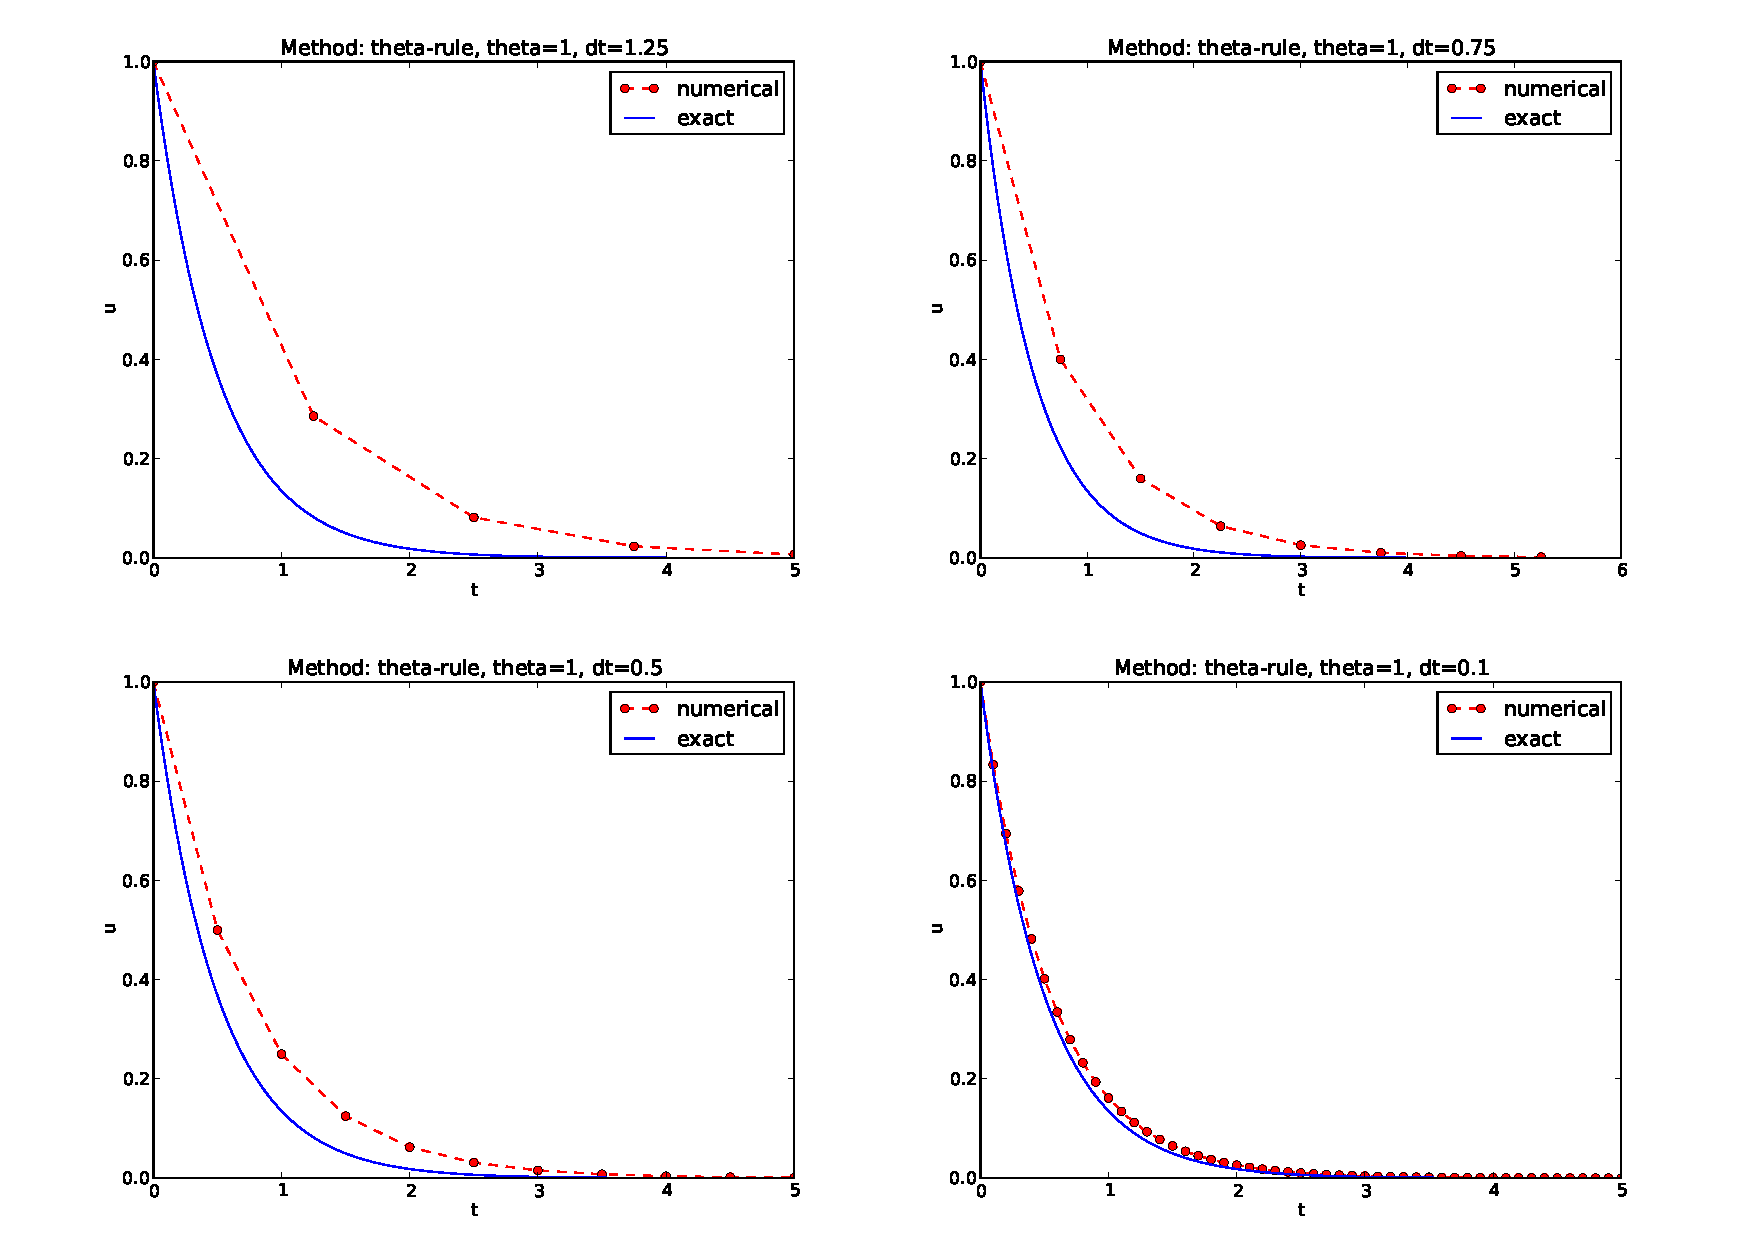
\includegraphics[width=1.1\linewidth]{fig-analysis/BE4c.pdf}}
  \caption{
  Backward Euler. \label{decay:analysis:BE4c}
  }
\end{figure}
%\clearpage % flush figures decay:analysis:BE4c



\begin{figure}[!ht]  % decay:analysis:CN4c
  \centerline{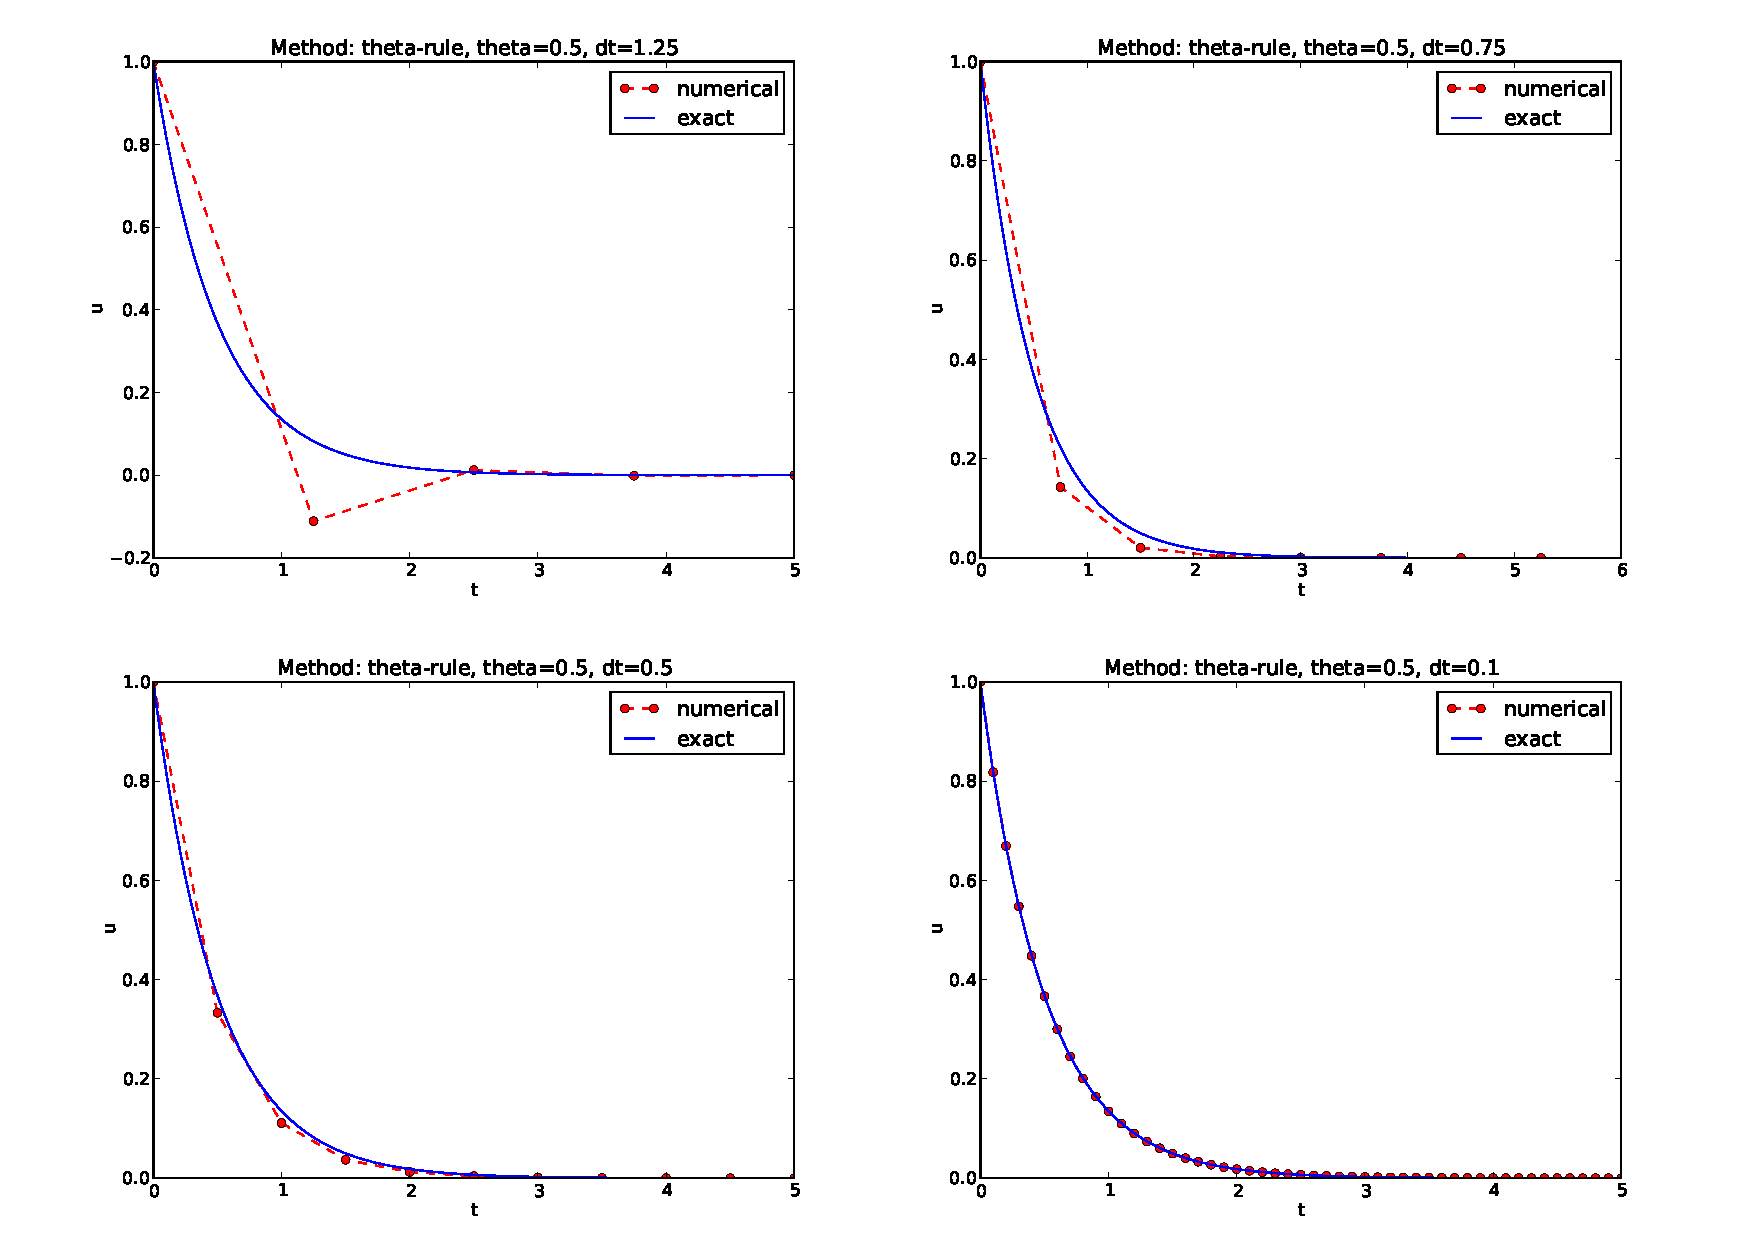
\includegraphics[width=1.1\linewidth]{fig-analysis/CN4c.pdf}}
  \caption{
  Crank-Nicolson. \label{decay:analysis:CN4c}
  }
\end{figure}
%\clearpage % flush figures decay:analysis:CN4c



\begin{figure}[!ht]  % decay:analysis:FE4c
  \centerline{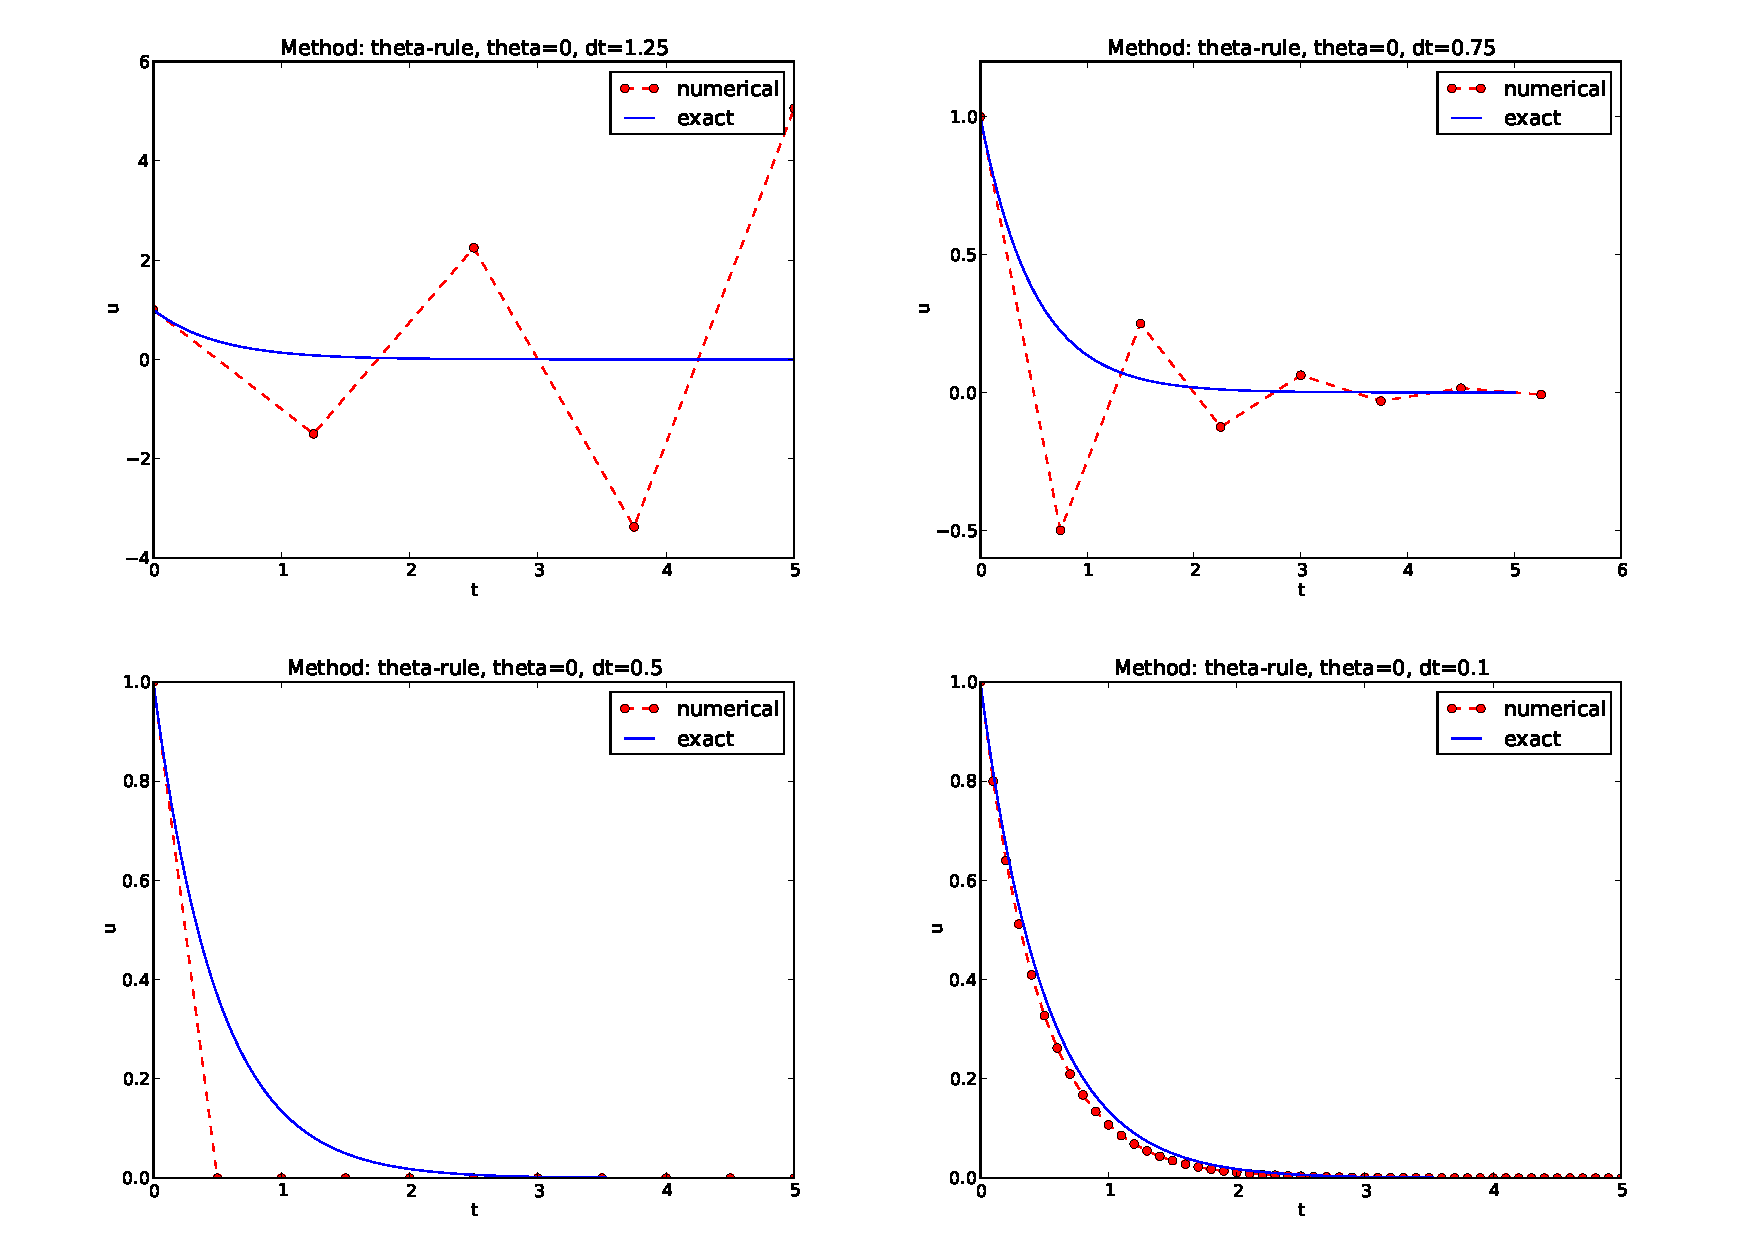
\includegraphics[width=1.1\linewidth]{fig-analysis/FE4c.pdf}}
  \caption{
  Forward Euler. \label{decay:analysis:FE4c}
  }
\end{figure}
%\clearpage % flush figures decay:analysis:FE4c


The characteristics of the displayed curves can be summarized as follows:

\begin{itemize}
  \item The Backward Euler scheme gives a monotone solution in all cases,
    lying above the exact curve.

  \item The Crank-Nicolson scheme gives the most accurate results, but for
    $\Delta t=1.25$ the solution oscillates.

  \item The Forward Euler scheme gives a growing, oscillating solution for
    $\Delta t=1.25$; a decaying, oscillating solution for $\Delta t=0.75$;
    a strange solution $u^n=0$ for $n\geq 1$ when $\Delta t=0.5$; and
    a solution seemingly as accurate as the one by the Backward Euler
    scheme for $\Delta t = 0.1$, but the curve lies below the exact
    solution.
\end{itemize}

\noindent
Since the exact solution of our model problem is a monotone function,
$u(t)=Ie^{-at}$, some of these qualitatively wrong results indeed seem alarming!


\begin{notice_mdfboxadmon}[Key questions.]

\begin{itemize}
 \item Under what circumstances, i.e., values of
   the input data $I$, $a$, and $\Delta t$ will the Forward Euler and
   Crank-Nicolson schemes result in undesired oscillatory solutions?

 \item How does $\Delta t$ impact the error in the numerical solution?
\end{itemize}

\noindent
The first question will be investigated both by numerical experiments and
by precise mathematical theory. The theory will help establish
general criteria on $\Delta t$ for avoiding non-physical oscillatory
or growing solutions.

For our simple model problem we can answer the second
question very precisely, but
we will also look at simplified formulas for small $\Delta t$
and touch upon important concepts such as \emph{convergence rate} and
\emph{the order of a scheme}. Other fundamental concepts mentioned are
stability, consistency, and convergence.
\end{notice_mdfboxadmon}



\subsection{Detailed experiments}

To address the first question above,
we may set up an experiment where we loop over values of $I$, $a$,
and $\Delta t$ in our chosen model problem.
For each experiment, we flag the solution as
oscillatory if

\[ u^{n} > u^{n-1},\]
for some value of $n$. This seems like a reasonable choice,
since we expect $u^n$ to decay with $n$, but oscillations will make
$u$ increase over a time step. Doing some initial experimentation
with varying $I$, $a$, and $\Delta t$, quickly reveals that
oscillations are independent of $I$, but they do depend on $a$ and
$\Delta t$. We can therefore limit the investigation to
vary $a$ and $\Delta t$. Based on this observation,
we introduce a two-dimensional
function $B(a,\Delta t)$ which is 1 if oscillations occur
and 0 otherwise. We can visualize $B$ as a contour plot
(lines for which $B=\hbox{const}$). The contour $B=0.5$
corresponds to the borderline between oscillatory regions with $B=1$
and monotone regions with $B=0$ in the $a,\Delta t$ plane.

The $B$ function is defined at discrete $a$ and $\Delta t$ values.
Say we have given $P$ values for $a$, $a_0,\ldots,a_{P-1}$, and
$Q$ values for $\Delta t$, $\Delta t_0,\ldots,\Delta t_{Q-1}$.
These $a_i$ and $\Delta t_j$ values, $i=0,\ldots,P-1$,
$j=0,\ldots,Q-1$, form a rectangular mesh of $P\times Q$ points
in the plane spanned by $a$ and $\Delta t$.
At each point $(a_i, \Delta t_j)$, we associate
the corresponding value $B(a_i,\Delta t_j)$, denoted $B_{ij}$.
The $B_{ij}$ values are naturally stored in a two-dimensional
array. We can thereafter create a plot of the
contour line $B_{ij}=0.5$ dividing the oscillatory and monotone
regions. The file \href{{http://tinyurl.com/ofkw6kc/analysis/decay_osc_regions.py}}{\nolinkurl{decay_osc_regions.py}}  given below (\Verb!osc_regions! stands for ``oscillatory regions'') contains all nuts and
bolts to produce the $B=0.5$ line in Figures~\ref{decay:analysis:B:FE}
and~\ref{decay:analysis:B:CN}. The oscillatory region is above this line.

\begin{pro}{cbg_blue1}{bar_blue1}\begin{Verbatim}[numbers=none,fontsize=\fontsize{9pt}{9pt},baselinestretch=0.95,xleftmargin=2mm]
from decay_mod import solver
import numpy as np
import scitools.std as st

def non_physical_behavior(I, a, T, dt, theta):
    """
    Given lists/arrays a and dt, and numbers I, dt, and theta,
    make a two-dimensional contour line B=0.5, where B=1>0.5
    means oscillatory (unstable) solution, and B=0<0.5 means
    monotone solution of u'=-au.
    """
    a = np.asarray(a); dt = np.asarray(dt)  # must be arrays
    B = np.zeros((len(a), len(dt)))         # results
    for i in range(len(a)):
        for j in range(len(dt)):
            u, t = solver(I, a[i], T, dt[j], theta)
            # Does u have the right monotone decay properties?
            correct_qualitative_behavior = True
            for n in range(1, len(u)):
                if u[n] > u[n-1]:  # Not decaying?
                    correct_qualitative_behavior = False
                    break  # Jump out of loop
            B[i,j] = float(correct_qualitative_behavior)
    a_, dt_ = st.ndgrid(a, dt)  # make mesh of a and dt values
    st.contour(a_, dt_, B, 1)
    st.grid('on')
    st.title('theta=%g' % theta)
    st.xlabel('a'); st.ylabel('dt')
    st.savefig('osc_region_theta_%s.png' % theta)
    st.savefig('osc_region_theta_%s.pdf' % theta)

non_physical_behavior(
    I=1,
    a=np.linspace(0.01, 4, 22),
    dt=np.linspace(0.01, 4, 22),
    T=6,
    theta=0.5)
\end{Verbatim}
\end{pro}
\noindent


\begin{figure}[!ht]  % decay:analysis:B:FE
  \centerline{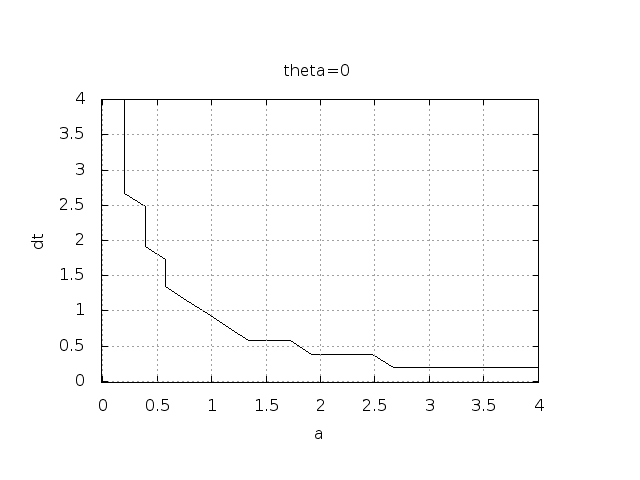
\includegraphics[width=0.9\linewidth]{fig-analysis/osc_region_FE.png}}
  \caption{
  Forward Euler scheme: oscillatory solutions occur for points above the curve. \label{decay:analysis:B:FE}
  }
\end{figure}
%\clearpage % flush figures decay:analysis:B:FE



\begin{figure}[!ht]  % decay:analysis:B:CN
  \centerline{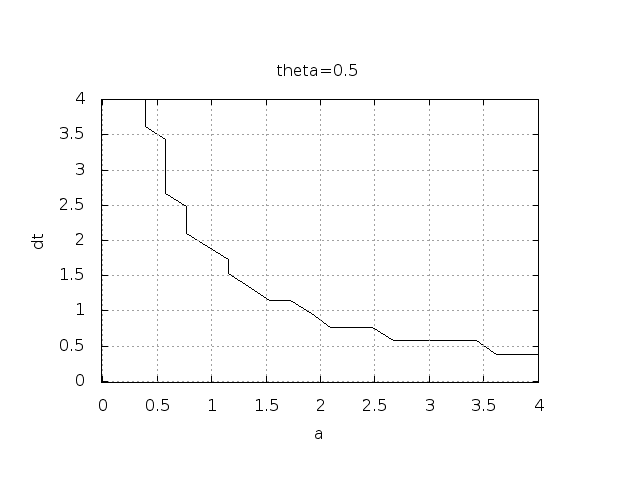
\includegraphics[width=0.9\linewidth]{fig-analysis/osc_region_CN.png}}
  \caption{
  Crank-Nicolson scheme: oscillatory solutions occur for points above the curve. \label{decay:analysis:B:CN}
  }
\end{figure}
%\clearpage % flush figures decay:analysis:B:CN


By looking at the curves in the figures one may guess that $a\Delta t$
must be less than a critical limit to avoid the undesired
oscillations.  This limit seems to be about 2 for Crank-Nicolson and 1
for Forward Euler.  We shall now establish a precise mathematical
analysis of the discrete model that can explain the observations in
our numerical experiments.


\section{Stability}

The goal now is to understand the results in the previous section.
To this end, we shall investigate the properties of the mathematical
formula for the solution of the equations arising from the finite
difference methods.

\subsection{Exact numerical solution}

Starting with $u^0=I$, the simple recursion (\ref{decay:analysis:scheme})
can be applied repeatedly $n$ times, with the result that
\begin{equation}
u^{n} = IA^n,\quad A = \frac{1 - (1-\theta) a\Delta t}{1 + \theta a\Delta t}\tp
\label{decay:analysis:unex}
\end{equation}


\begin{notice_mdfboxadmon}[Solving difference equations.]
Difference equations where all terms are linear in
$u^{n+1}$, $u^n$, and maybe $u^{n-1}$, $u^{n-2}$, etc., are
called \emph{homogeneous, linear} difference equations, and their solutions
are generally of the form $u^n=A^n$, where $A$ is a constant to be
determined. Inserting this expression in the difference equation
and dividing by $A^{n+1}$ gives
a polynomial equation in $A$. In the present case we get

\[ A = \frac{1 - (1-\theta) a\Delta t}{1 + \theta a\Delta t}\tp \]
This is a solution technique of wider applicability than repeated use of
the recursion (\ref{decay:analysis:scheme}).
\end{notice_mdfboxadmon}



Regardless of the solution approach, we have obtained a formula for
$u^n$.  This formula can explain everything we see in the figures
above, but it also gives us a more general insight into accuracy and
stability properties of the three schemes.

\index{stability}

Since $u^n$ is a factor $A$
raised to an integer power $n$, we realize that $A < 0$
will imply $u^n < 0$ for odd $n$ and $u^n > 0$ for even $n$.
That is, the solution oscillates between the mesh points.
We have oscillations due to $A < 0$ when

\begin{equation}
(1-\theta)a\Delta t > 1 \tp
\label{decay:th:stability}
\end{equation}
Since $A>0$ is a requirement for having a numerical solution with the
same basic property (monotonicity) as the exact solution, we may say
that $A>0$ is a \emph{stability criterion}. Expressed in terms of $\Delta t$
the stability criterion reads

\begin{equation}
\Delta t < \frac{1}{(1-\theta)a}\tp
\end{equation}

The Backward
Euler scheme is always stable since $A < 0$ is impossible for $\theta=1$, while
non-oscillating solutions for Forward Euler and Crank-Nicolson
demand $\Delta t\leq 1/a$ and $\Delta t\leq 2/a$, respectively.
The relation between $\Delta t$ and $a$ look reasonable: a larger
$a$ means faster decay and hence a need for smaller time steps.

Looking at the upper left plot in Figure~\ref{decay:analysis:FE4c},
we see that $\Delta t=1.25$, and remembering that $a=2$ in these
experiments, $A$ can be calculated to be
$-1.5$, so the Forward Euler solution becomes $u^n=(-1.5)^n$ ($I=1$).
This solution oscillates \emph{and} grows. The upper right plot has
$a\Delta t = 2\cdot 0.75=1.5$, so $A=-0.5$,
and $u^n=(-0.5)^n$ decays but oscillates. The lower left plot
is a peculiar case where the Forward Euler scheme produces a solution
that is stuck on the $t$ axis. Now we can understand why this is so,
because $a\Delta t= 2\cdot 0.5=1$, which gives $A=0$,
and therefore $u^n=0$ for $n\geq 1$.  The decaying oscillations in the Crank-Nicolson scheme in the upper left plot in Figure~\ref{decay:analysis:CN4c}
for $\Delta t=1.25$ are easily explained by the fact that $A\approx -0.11 < 0$.


\subsection{Stability properties derived from the amplification factor}
\index{amplification factor}

The factor $A$ is called the \emph{amplification factor} since the solution
at a new time level is the solution at the previous time
level amplified by a factor $A$.
For a decay process, we must obviously have $|A|\leq 1$, which
is fulfilled for all $\Delta t$ if $\theta \geq 1/2$. Arbitrarily
large values of $u$ can be generated when $|A|>1$ and $n$ is large
enough. The numerical solution is in such cases totally irrelevant to
an ODE modeling decay processes! To avoid this situation, we must
demand $|A|\leq 1$ also for $\theta < 1/2$, which implies

\begin{equation}
\Delta t \leq \frac{2}{(1-2\theta)a},
\end{equation}
For example, $\Delta t$ must not exceed  $2/a$ when computing with
the Forward Euler scheme.

\index{A-stable methods}
\index{L-stable methods}


\begin{notice_mdfboxadmon}[Stability properties.]
We may summarize the stability investigations as follows:

\begin{enumerate}
\item The Forward Euler method is a \emph{conditionally stable} scheme because
   it requires $\Delta t < 2/a$ for avoiding growing solutions
   and $\Delta t < 1/a$ for avoiding oscillatory solutions.

\item The Crank-Nicolson is \emph{unconditionally stable} with respect to
   growing solutions, while it is conditionally stable with
   the criterion $\Delta t < 2/a$ for avoiding oscillatory solutions.

\item The Backward Euler method is unconditionally stable with respect
   to growing and oscillatory solutions - any $\Delta t$ will work.
\end{enumerate}

\noindent
Much literature on ODEs speaks about L-stable and A-stable methods.
In our case A-stable methods ensures non-growing solutions, while
L-stable methods also avoids oscillatory solutions.
\end{notice_mdfboxadmon}



\section{Accuracy}

While stability concerns the qualitative properties of the numerical
solution, it remains to investigate the quantitative properties to
see exactly how large the numerical errors are.

\subsection{Visual comparison of amplification factors}

After establishing how $A$ impacts the qualitative features of the
solution, we shall now look more into how well the numerical amplification
factor approximates the exact one. The exact solution reads
$u(t)=Ie^{-at}$, which can be rewritten as
\begin{equation}
{\uex}(t_n) = Ie^{-a n\Delta t} = I(e^{-a\Delta t})^n \tp
\end{equation}
From this formula we see that the exact amplification factor is
\begin{equation}
\Aex = e^{-a\Delta t} \tp
\end{equation}

We see from all of our analysis
that the exact and numerical amplification factors depend
on $a$ and $\Delta t$ through the dimensionless
product $a\Delta t$: whenever there is a
$\Delta t$ in the analysis, there is always an associated $a$
parameter. Therefore, it
is convenient to introduce a symbol for this product, $p=a\Delta t$,
and view $A$ and $\Aex$ as functions of $p$. Figure~\ref{decay:analysis:fig:A} shows these functions. The two amplification
factors are clearly closest for the
Crank-Nicolson method, but that method has
the unfortunate oscillatory behavior when $p>2$.


\begin{figure}[!ht]  % decay:analysis:fig:A
  \centerline{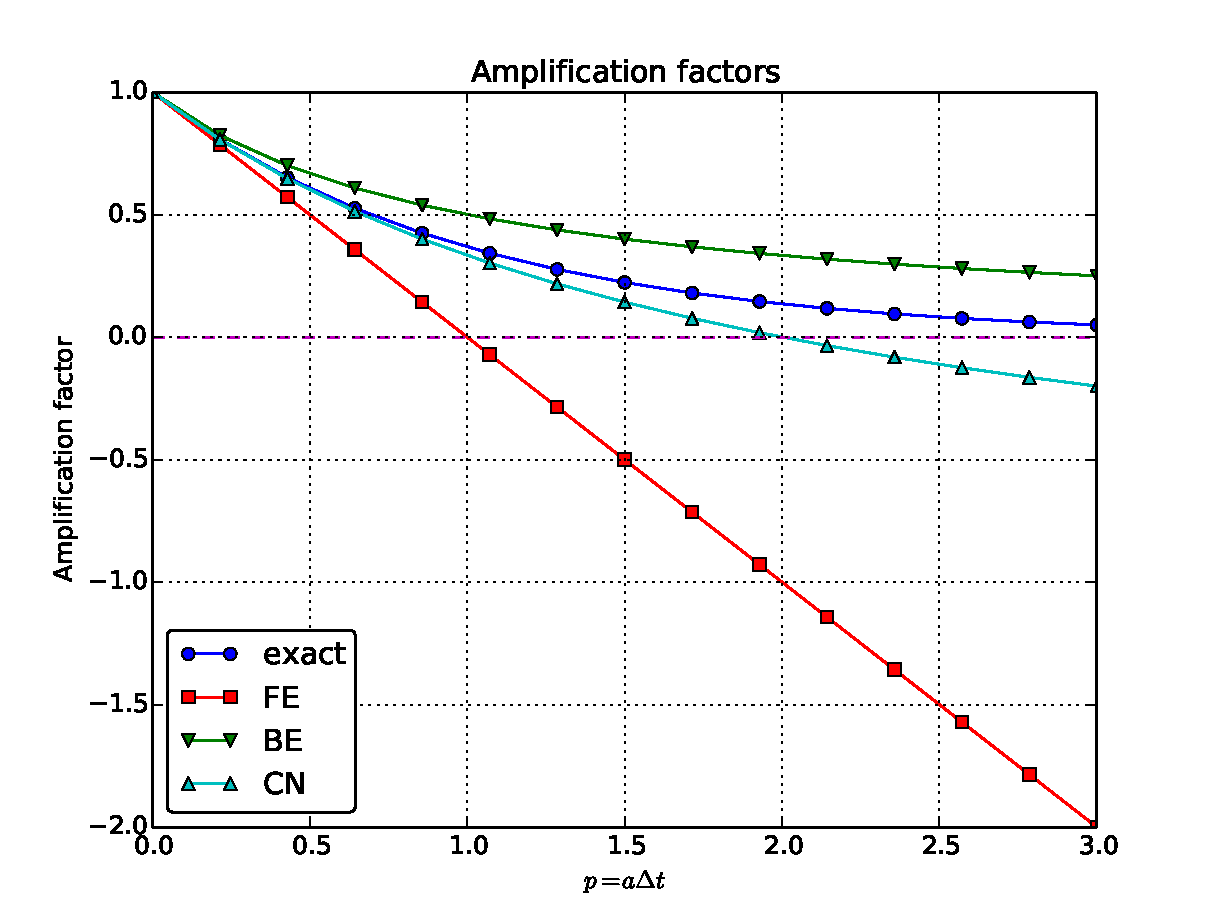
\includegraphics[width=0.9\linewidth]{fig-analysis/A_factors.pdf}}
  \caption{
  Comparison of amplification factors. \label{decay:analysis:fig:A}
  }
\end{figure}
%\clearpage % flush figures decay:analysis:fig:A




\begin{notice_mdfboxadmon}[Significance of the $p=a\Delta t$ parameter.]
The key parameter for numerical performance of a scheme is in this model
problem $p=a\Delta t$. This is a \emph{dimensionless number} ($a$ has dimension
1/s and $\Delta t$ has dimension s) reflecting how the discretization
parameter plays together with a physical parameter in the problem.

One can bring the present model problem on dimensionless form
through a process called scaling. The scaled modeled has a modified
time $\bar t = at$ and modified response $\bar u =u/I$ such that
the model reads $d\bar u/d\bar t = -\bar u$, $\bar u(0)=1$.
Analyzing this model, where there are no physical parameters,
we find that $\Delta \bar t$ is the key parameter
for numerical performance. In the unscaled model,
this corresponds to $\Delta \bar t = a\Delta t$.

It is common that the numerical performance of methods for solving ordinary and
partial differential equations is governed by dimensionless parameters
that combine mesh sizes with physical parameters.
\end{notice_mdfboxadmon}



\subsection{Series expansion of amplification factors}

As an alternative to the visual understanding inherent in Figure~\ref{decay:analysis:fig:A}, there is a strong tradition in numerical
analysis to establish formulas for approximation errors when the
discretization parameter, here $\Delta t$, becomes small. In the
present case, we let $p$ be our small discretization parameter, and it
makes sense to simplify the expressions for $A$ and $\Aex$ by using
Taylor polynomials around $p=0$.  The Taylor polynomials are accurate
for small $p$ and greatly simplify the comparison of the analytical
expressions since we then can compare polynomials, term by term.

Calculating the Taylor series for $\Aex$ is easily done by hand, but
the three versions of $A$ for $\theta=0,1,{\half}$ lead to more
cumbersome calculations.
Nowadays, analytical computations can benefit greatly by
symbolic computer algebra software. The Python package \texttt{sympy}
represents a powerful computer algebra system, not yet as sophisticated as
the famous Maple and Mathematica systems, but it is free and
very easy to integrate with our numerical computations in Python.

\index{interactive Python}
\index{isympy@{\rm\texttt{isympy}}}
\index{sympy@{\rm\texttt{sympy}}}

When using \texttt{sympy}, it is convenient to enter an interactive Python
shell where the results of expressions and statements can be shown
immediately.
Here is a simple example. We strongly recommend to use
\texttt{isympy} (or \texttt{ipython}) for such interactive sessions.

Let us illustrate \texttt{sympy} with a standard Python shell syntax
(\texttt{>>>} prompt) to compute a Taylor polynomial approximation to $e^{-p}$:

\begin{cod}{cbg_blue1}\begin{Verbatim}[numbers=none,fontsize=\fontsize{9pt}{9pt},baselinestretch=0.95,xleftmargin=2mm]
>>> from sympy import *
>>> # Create p as a mathematical symbol with name 'p'
>>> p = Symbol('p')
>>> # Create a mathematical expression with p
>>> A_e = exp(-p)
>>>
>>> # Find the first 6 terms of the Taylor series of A_e
>>> A_e.series(p, 0, 6)
1 + (1/2)*p**2 - p - 1/6*p**3 - 1/120*p**5 + (1/24)*p**4 + O(p**6)
\end{Verbatim}
\end{cod}
\noindent
Lines with \texttt{>>>} represent input lines, whereas without
this prompt represent the result of the previous command (note that
\texttt{isympy} and \texttt{ipython} apply other prompts, but in this text
we always apply \texttt{>>>} for interactive Python computing).
Apart from the order of the powers, the computed formula is easily
recognized as the beginning of the Taylor series for $e^{-p}$.

Let us define the numerical amplification factor where $p$ and $\theta$
enter the formula as symbols:
\begin{cod}{cbg_blue1}\begin{Verbatim}[numbers=none,fontsize=\fontsize{9pt}{9pt},baselinestretch=0.95,xleftmargin=2mm]
>>> theta = Symbol('theta')
>>> A = (1-(1-theta)*p)/(1+theta*p)
\end{Verbatim}
\end{cod}
\noindent
To work with the factor for the Backward Euler scheme we
can substitute the value 1 for \texttt{theta}:

\begin{cod}{cbg_blue1}\begin{Verbatim}[numbers=none,fontsize=\fontsize{9pt}{9pt},baselinestretch=0.95,xleftmargin=2mm]
>>> A.subs(theta, 1)
1/(1 + p)
\end{Verbatim}
\end{cod}
\noindent
Similarly, we can substitute \texttt{theta} by 1/2 for Crank-Nicolson,
preferably using an exact rational representation of 1/2 in \texttt{sympy}:

\begin{cod}{cbg_blue1}\begin{Verbatim}[numbers=none,fontsize=\fontsize{9pt}{9pt},baselinestretch=0.95,xleftmargin=2mm]
>>> half = Rational(1,2)
>>> A.subs(theta, half)
1/(1 + (1/2)*p)*(1 - 1/2*p)
\end{Verbatim}
\end{cod}
\noindent

The Taylor series of the amplification factor for the Crank-Nicolson
scheme can be computed as

\begin{cod}{cbg_blue1}\begin{Verbatim}[numbers=none,fontsize=\fontsize{9pt}{9pt},baselinestretch=0.95,xleftmargin=2mm]
>>> A.subs(theta, half).series(p, 0, 4)
1 + (1/2)*p**2 - p - 1/4*p**3 + O(p**4)
\end{Verbatim}
\end{cod}
\noindent
We are now in a position to compare Taylor series:

\begin{cod}{cbg_blue1}\begin{Verbatim}[numbers=none,fontsize=\fontsize{9pt}{9pt},baselinestretch=0.95,xleftmargin=2mm]
>>> FE = A_e.series(p, 0, 4) - A.subs(theta, 0).series(p, 0, 4)
>>> BE = A_e.series(p, 0, 4) - A.subs(theta, 1).series(p, 0, 4)
>>> CN = A_e.series(p, 0, 4) - A.subs(theta, half).series(p, 0, 4 )
>>> FE
(1/2)*p**2 - 1/6*p**3 + O(p**4)
>>> BE
-1/2*p**2 + (5/6)*p**3 + O(p**4)
>>> CN
(1/12)*p**3 + O(p**4)
\end{Verbatim}
\end{cod}
\noindent
From these expressions we see that the error $A-\Aex\sim \Oof{p^2}$
for the Forward and Backward Euler schemes, while
$A-\Aex\sim \Oof{p^3}$ for the Crank-Nicolson scheme.
The notation $\Oof{p^m}$ here means a polynomial in $p$ where
$p^m$ is the term of lowest-degree, and consequently the term that
dominates the expression for $p < 0$. We call this the
\emph{leading order term}. As $p\rightarrow 0$, the leading order term
clearly dominates over the higher-order terms (think of $p=0.01$:
$p$ is a hundred times larger than $p^2$).

Now, $a$ is a given parameter in the problem, while $\Delta t$ is
what we can vary. Not surprisingly, the error expressions are usually
written in terms $\Delta t$. We then have

\begin{equation}
A-\Aex = \left\lbrace\begin{array}{ll}
\Oof{\Delta t^2}, & \hbox{Forward and Backward Euler},\\ 
\Oof{\Delta t^3}, & \hbox{Crank-Nicolson}
\end{array}\right.
\end{equation}

We say that the Crank-Nicolson scheme has an error in the amplification
factor of order $\Delta t^3$, while the two other schemes are
of order $\Delta t^2$ in the same quantity.

What is the significance of the order expression? If we halve $\Delta t$,
the error in amplification factor at a time level will be reduced
by a factor of 4 in the Forward and Backward Euler schemes, and by
a factor of 8 in the Crank-Nicolson scheme. That is, as we
reduce $\Delta t$ to obtain more accurate results, the Crank-Nicolson
scheme reduces the error more efficiently than the other schemes.


\subsection{The ratio of numerical and exact amplification factors}

\index{error!amplification factor}

An alternative comparison of the schemes is provided by looking at the
ratio $A/\Aex$, or the error $1-A/\Aex$ in this ratio:

\begin{cod}{cbg_blue1}\begin{Verbatim}[numbers=none,fontsize=\fontsize{9pt}{9pt},baselinestretch=0.95,xleftmargin=2mm]
>>> FE = 1 - (A.subs(theta, 0)/A_e).series(p, 0, 4)
>>> BE = 1 - (A.subs(theta, 1)/A_e).series(p, 0, 4)
>>> CN = 1 - (A.subs(theta, half)/A_e).series(p, 0, 4)
>>> FE
(1/2)*p**2 + (1/3)*p**3 + O(p**4)
>>> BE
-1/2*p**2 + (1/3)*p**3 + O(p**4)
>>> CN
(1/12)*p**3 + O(p**4)
\end{Verbatim}
\end{cod}
\noindent
The leading-order terms have the same powers as
in the analysis of $A-\Aex$.

\subsection{The global error at a point}
\label{decay:analysis:gobal:error}

\index{error!global}

The error in the amplification factor reflects the error when
progressing from time level $t_n$ to $t_{n-1}$ only. That is,
we disregard the error already present in the solution at $t_{n-1}$.
The real error at a point, however, depends on the error development
over all previous time steps. This error,
$e^n = u^n-\uex(t_n)$, is known as the \emph{global error}. We
may look at $u^n$ for some $n$ and Taylor expand the
mathematical expressions as functions of $p=a\Delta t$ to get a simple
expression for the global error (for small $p$):

\begin{cod}{cbg_blue1}\begin{Verbatim}[numbers=none,fontsize=\fontsize{9pt}{9pt},baselinestretch=0.95,xleftmargin=2mm]
>>> n = Symbol('n')
>>> u_e = exp(-p*n)
>>> u_n = A**n
>>> FE = u_e.series(p, 0, 4) - u_n.subs(theta, 0).series(p, 0, 4)
>>> BE = u_e.series(p, 0, 4) - u_n.subs(theta, 1).series(p, 0, 4)
>>> CN = u_e.series(p, 0, 4) - u_n.subs(theta, half).series(p, 0, 4)
>>> FE
(1/2)*n*p**2 - 1/2*n**2*p**3 + (1/3)*n*p**3 + O(p**4)
>>> BE
(1/2)*n**2*p**3 - 1/2*n*p**2 + (1/3)*n*p**3 + O(p**4)
>>> CN
(1/12)*n*p**3 + O(p**4)
\end{Verbatim}
\end{cod}
\noindent
Note that \texttt{sympy} does not sort the polynomial terms in the output,
so $p^3$ appears before $p^2$ in the output of \texttt{BE}.

For a fixed time $t$, the parameter $n$ in these expressions increases
as $p\rightarrow 0$ since $t=n\Delta t =\mbox{const}$ and hence
$n$ must increase like $\Delta t^{-1}$. With $n$ substituted by
$t/\Delta t$ in
the leading-order error terms, these become

\begin{align}
e^n &= \half n p^2 = {\half}ta^2\Delta t, &\hbox{Forward Euler}
\label{decay:analysis:gobal:error:FE}\\ 
e^n &= -\half n p^2 = -{\half}ta^2\Delta t, &\hbox{Backward Euler}
\label{decay:analysis:gobal:error:BE}\\ 
e^n &= \frac{1}{12}np^3 = \frac{1}{12}ta^3\Delta t^2, &\hbox{Crank-Nicolson}
\label{decay:analysis:gobal:error:CN}
\end{align}
The global error is therefore of
second order (in $\Delta t$) for the Crank-Nicolson scheme and of
first order for the other two schemes.


\begin{notice_mdfboxadmon}[Convergence.]
When the global error $e^n\rightarrow 0$ as $\Delta t\rightarrow 0$,
we say that the scheme is \emph{convergent}. It means that the numerical
solution approaches the exact solution as the mesh is refined, and
this is a much desired property of a numerical method.
\end{notice_mdfboxadmon}



\subsection{Integrated error}
\label{decay:analysis:gobal:error_int}

The $L^2$ norm of the error can be computed by treating $e^n$ as a function
of $t$ in \texttt{sympy} and performing symbolic integration. For
the Forward Euler scheme we have

\begin{cod}{cbg_blue1}\begin{Verbatim}[numbers=none,fontsize=\fontsize{9pt}{9pt},baselinestretch=0.95,xleftmargin=2mm]
p, n, a, dt, t, T, theta = symbols('p n a dt t T 'theta')
A = (1-(1-theta)*p)/(1+theta*p)
u_e = exp(-p*n)
u_n = A**n
error = u_e.series(p, 0, 4) - u_n.subs(theta, 0).series(p, 0, 4)
# Introduce t and dt instead of n and p
error = error.subs('n', 't/dt').subs(p, 'a*dt')
error = error.as_leading_term(dt) # study only the first term
print error
error_L2 = sqrt(integrate(error**2, (t, 0, T)))
print error_L2
\end{Verbatim}
\end{cod}
\noindent
The output reads

\begin{cod}{cbg_blue1}\begin{Verbatim}[numbers=none,fontsize=\fontsize{9pt}{9pt},baselinestretch=0.95,xleftmargin=2mm]
sqrt(30)*sqrt(T**3*a**4*dt**2*(6*T**2*a**2 - 15*T*a + 10))/60
\end{Verbatim}
\end{cod}
\noindent
which means that the $L^2$ error behaves like $a^2\Delta t$.

Strictly speaking, the numerical error is only defined at the
mesh points so it makes most sense to compute the
$\ell^2$ error

\[ ||e^n||_{\ell^2} = \sqrt{\Delta t\sum_{n=0}^{N_t} ({\uex}(t_n) - u^n)^2}
\tp \]
We have obtained an exact analytical expression for the error at
$t=t_n$, but here we use the leading-order error term only since we
are mostly interested in how the error behaves as a polynomial in
$\Delta t$ or $p$, and then the leading order term will dominate.  For
the Forward Euler scheme, $\uex(t_n) - u^n \approx {\half}np^2$, and
we have

\[
||e^n||_{\ell^2}^2 = \Delta t\sum_{n=0}^{N_t} \frac{1}{4}n^2p^4
=\Delta t\frac{1}{4}p^4 \sum_{n=0}^{N_t} n^2\tp
\]
Now, $\sum_{n=0}^{N_t} n^2\approx \frac{1}{3}N_t^3$. Using this approximation,
setting $N_t =T/\Delta t$, and taking the square root gives the expression

\begin{equation}
||e^n||_{\ell^2} = \half\sqrt{\frac{T^3}{3}} a^2\Delta t\tp
\label{decay:analysis:gobal:error_int:FE}
\end{equation}
Calculations for the Backward Euler scheme are very similar and provide
the same result, while the Crank-Nicolson scheme leads to

\begin{equation}
||e^n||_{\ell^2} = \frac{1}{12}\sqrt{\frac{T^3}{3}}a^3\Delta t^2\tp
\label{decay:analysis:gobal:error_int:CN}
\end{equation}


\begin{summary_mdfboxadmon}[Summary of errors.]
Both the global point-wise errors (\ref{decay:analysis:gobal:error:FE})-(\ref{decay:analysis:gobal:error:CN})
and their time-integrated versions (\ref{decay:analysis:gobal:error_int:FE}) and (\ref{decay:analysis:gobal:error_int:CN}) show that

\begin{itemize}
 \item the Crank-Nicolson scheme is of second order in $\Delta t$, and

 \item the Forward Euler and Backward Euler schemes are of first order in $\Delta t$.
\end{itemize}

\noindent
\end{summary_mdfboxadmon}



\subsection{Truncation error}
\label{decay:analysis:trunc}

The truncation error is a very frequently used error measure for
finite difference methods. It is defined as \emph{the error
in the difference equation that arises when inserting the exact
solution}. Contrary to many other error measures, e.g., the
true error $e^n=\uex(t_n)-u^n$, the truncation error is a quantity that
is easily computable.


Let us illustrate the calculation of the truncation error
for the Forward Euler scheme.
We start with the difference equation on operator form,

\[ \lbrack D_t^+ u = -au\rbrack^n,\]
which is the short form for

\[ \frac{u^{n+1}-u^n}{\Delta t} = -au^n\tp\]
The idea is to see how well the exact solution $\uex(t)$ fulfills
this equation. Since $\uex(t)$ in general will not obey the
discrete equation, we get an error in the discrete equation. This
error is called
a \emph{residual}, denoted here by $R^n$:

\begin{equation}
R^n = \frac{\uex(t_{n+1})-\uex(t_n)}{\Delta t} + a\uex(t_n)
\tp
\label{decay:analysis:trunc:Req}
\end{equation}
The residual is defined at each mesh point and is therefore a mesh
function with a superscript $n$.

The interesting feature of $R^n$ is to see how it
depends on the discretization parameter $\Delta t$.
The tool for reaching
this goal is to Taylor expand $\uex$ around the point where the
difference equation is supposed to hold, here $t=t_n$.
We have that

\[ \uex(t_{n+1}) = \uex(t_n) + \uex'(t_n)\Delta t + \half\uex''(t_n)
\Delta t^2 + \cdots, \]
which may be used to reformulate the fraction in
(\ref{decay:analysis:trunc:Req}) so that

\[ R^n = \uex'(t_n) + \half\uex''(t_n)\Delta t + \ldots + a\uex(t_n)\tp\]
Now, $\uex$ fulfills the ODE $\uex'=-a\uex$, which means that the first and last
term cancel and we have

\[ R^n = \half\uex''(t_n)\Delta t + \Oof{\Delta t^2}\tp \]
This $R^n$ is the \emph{truncation error}, which for the Forward Euler is seen
to be of first order in $\Delta t$ as $\Delta \rightarrow 0$.

The above procedure can be repeated for the Backward Euler and the
Crank-Nicolson schemes. We start with the scheme in operator notation,
write it out in detail, Taylor expand $\uex$ around the point $\tilde t$
at which the difference equation is defined, collect terms that
correspond to the ODE (here $\uex' + a\uex$), and identify the remaining
terms as the residual $R$, which is the truncation error.
The Backward Euler scheme leads to

\[ R^n \approx -\half\uex''(t_n)\Delta t, \]
while the Crank-Nicolson scheme gives

\[ R^{n+\half} \approx \frac{1}{24}\uex'''(t_{n+\half})\Delta t^2,\]
when $\Delta t\rightarrow 0$.

The \emph{order} $r$ of a finite difference scheme is often defined through
the leading term $\Delta t^r$ in the truncation error. The above
expressions point out that the Forward and Backward Euler schemes are
of first order, while Crank-Nicolson is of second order.  We have
looked at other error measures in other sections, like the error in
amplification factor and the error $e^n=\uex(t_n)-u^n$, and expressed
these error measures in terms of $\Delta t$ to see the order of the
method. Normally, calculating the truncation error is more
straightforward than deriving the expressions for other error measures
and therefore the easiest way to establish the order of a scheme.

\subsection{Consistency, stability, and convergence}

\index{consistency} \index{stability} \index{convergence}

Three fundamental concepts when solving differential equations by
numerical methods are consistency, stability, and convergence.  We
shall briefly touch upon these concepts below in the context of the present
model problem.

Consistency means that the error in the difference equation, measured
through the truncation error, goes to zero as $\Delta t\rightarrow
0$. Since the truncation error tells how well the exact solution
fulfills the difference equation, and the exact solution fulfills the
differential equation, consistency ensures that the difference
equation approaches the differential equation in the limit. The
expressions for the truncation errors in the previous section are all
proportional to $\Delta t$ or $\Delta t^2$, hence they vanish as
$\Delta t\rightarrow 0$, and all the schemes are consistent.  Lack of
consistency implies that we actually solve some other differential
equation in the limit $\Delta t\rightarrow 0$ than we aim at.

Stability means that the numerical solution exhibits the same
qualitative properties as the exact solution. This is obviously a
feature we want the numerical solution to have. In the present
exponential decay model, the exact solution is monotone and
decaying. An increasing numerical solution is not in accordance with
the decaying nature of the exact solution and hence unstable. We can
also say that an oscillating numerical solution lacks the property of
monotonicity of the exact solution and is also unstable. We have seen
that the Backward Euler scheme always leads to monotone and decaying
solutions, regardless of $\Delta t$, and is hence stable. The Forward
Euler scheme can lead to increasing solutions and oscillating
solutions if $\Delta t$ is too large and is therefore unstable unless
$\Delta t$ is sufficiently small.  The Crank-Nicolson can never lead
to increasing solutions and has no problem to fulfill that stability
property, but it can produce oscillating solutions and is unstable in
that sense, unless $\Delta t$ is sufficiently small.

Convergence implies that the global (true) error mesh function $e^n =
\uex(t_n)-u^n\rightarrow 0$ as $\Delta t\rightarrow 0$. This is really
what we want: the numerical solution gets as close to the exact
solution as we request by having a sufficiently fine mesh.

Convergence is hard to establish theoretically, except in quite simple
problems like the present one. Stability and consistency are much
easier to calculate. A major breakthrough in the understanding of
numerical methods for differential equations came in 1956 when Lax and
Richtmeyer established equivalence between convergence on one hand and
consistency and stability on the other (the \href{{http://en.wikipedia.org/wiki/Lax_equivalence_theorem}}{Lax equivalence theorem}).  In practice
it meant that one can first establish that a method is stable and
consistent, and then it is automatically convergent (which is much
harder to establish).  The result holds for linear problems only, and
in the world of nonlinear differential equations the relations between
consistency, stability, and convergence are much more complicated.

We have seen in the previous analysis that the Forward Euler,
Backward Euler, and Crank-Nicolson schemes are convergent ($e^n\rightarrow 0$),
that they are consistent ($R^n\rightarrow 0$), and that they are
stable under certain conditions on the size of $\Delta t$.
We have also derived explicit mathematical expressions for $e^n$,
the truncation error, and the stability criteria.

% Look in Asher and Petzold, p 40

\section{Exercises}



% --- begin exercise ---
\begin{doconceexercise}
\refstepcounter{doconceexercisecounter}

\subsection*{Problem \thedoconceexercisecounter: Visualize the accuracy of finite differences}

\label{decay:analysis:exer:fd:exp:plot}

The purpose of this exercise is to visualize the accuracy of finite difference
approximations of the derivative of a given function.
For any finite difference approximation, take the Forward Euler difference
as an example, and any specific function, take  $u=e^{-at}$,
we may introduce an error fraction

\begin{align*}
E = \frac{[D_t^+ u]^n}{u'(t_n)} &= \frac{\exp{(-a(t_n+\Delta t))} - \exp{(-at_n)}}{-a\exp{(-at_n)\Delta t}}\\ 
&= \frac{1}{a\Delta t}\left(1 -\exp{(-a\Delta t)}\right),
\end{align*}
and view $E$ as a function of $\Delta t$. We expect that
$\lim_{\Delta t\rightarrow 0}E=1$, while $E$ may deviate significantly from
unity for large $\Delta t$. How the error depends on $\Delta t$ is best
visualized in a graph where we use a logarithmic scale for $\Delta t$,
so we can cover many orders of magnitude of that quantity. Here is
a code segment creating an array of 100 intervals, on the logarithmic
scale, ranging from $10^{-6}$ to $10^{-0.5}$ and then plotting $E$ versus
$p=a\Delta t$ with logarithmic scale on the $p$ axis:

\begin{cod}{cbg_blue1}\begin{Verbatim}[numbers=none,fontsize=\fontsize{9pt}{9pt},baselinestretch=0.95,xleftmargin=2mm]
from numpy import logspace, exp
from matplotlib.pyplot import semilogx
p = logspace(-6, -0.5, 101)
y = (1-exp(-p))/p
semilogx(p, y)
\end{Verbatim}
\end{cod}
\noindent
Illustrate such errors for the finite difference operators $[D_t^+u]^n$
(forward), $[D_t^-u]^n$ (backward), and $[D_t u]^n$ (centered) in
the same plot.

Perform a Taylor series expansions of the error fractions and find
the leading order $r$ in the expressions of type
$1 + Cp^r + \Oof{p^{r+1}}$, where $C$ is some constant.

% --- begin hint in exercise ---

\paragraph{Hint.}
To save manual calculations and learn more about symbolic computing,
make functions for the three difference operators and use \texttt{sympy}
to perform the symbolic differences, differentiation, and Taylor series
expansion. To plot a symbolic expression \texttt{E} against \texttt{p}, convert the
expression to a Python function first: \texttt{E = sympy.lamdify([p], E)}.

% --- end hint in exercise ---


% removed !bsol ... !esol environment (because of the command-line option --without_solutions)
\noindent Filename: \Verb!decay_plot_fd_error!.

\end{doconceexercise}
% --- end exercise ---




% --- begin exercise ---
\begin{doconceexercise}
\refstepcounter{doconceexercisecounter}

\subsection*{Problem \thedoconceexercisecounter: Explore the $\theta$-rule for exponential growth}

\label{decay:analysis:exer:growth}

This exercise asks you to solve the ODE $u'=-au$ with $a < 0$ such that
the ODE models exponential growth instead of exponential decay.  A
central theme is to investigate numerical artifacts and non-physical
solution behavior.


\subex{a)}
Set $a=-1$ and run experiments with $\theta=0, 0.5, 1$ for
various values of $\Delta t$ to uncover numerical artifacts.
Recall that the exact solution is a
monotone, growing function when $a < 0$. Oscillations or significantly
wrong growth are signs of wrong qualitative behavior.

From the experiments, select four values of $\Delta t$ that
demonstrate the kind of numerical solutions that are characteristic
for this model.


% removed !bsol ... !esol environment (because of the command-line option --without_solutions)

\subex{b)}
Write up the amplification factor and plot it for $\theta=0,0.5,1$
together with the exact one for $a\Delta t < 0$. Use the plot to
explain the observations made in the experiments.

% --- begin hint in exercise ---

\paragraph{Hint.}
Modify the \href{{http://tinyurl.com/ofkw6kc/analysis/decay_ampf_plot.py}}{\nolinkurl{decay_ampf_plot.py}} code
(in the \texttt{src/analysis} directory).

% --- end hint in exercise ---


% removed !bsol ... !esol environment (because of the command-line option --without_solutions)

\noindent Filename: \Verb!exponential_growth!.

\end{doconceexercise}
% --- end exercise ---


% !split


\bibliographystyle{plain}
\bibliography{../papers}

% ------------------- end of main content ---------------

% #ifdef PREAMBLE
\cleardoublepage\phantomsection  % trick to get correct link to Index
\printindex

\end{document}
% #endif

